\documentclass[oneside,12pt,pdftex]{Classes/uitBA}
\usepackage{mathptmx}
\usepackage{float}
\usepackage{fancyhdr}
\usepackage{pdfpages}
\usepackage{multirow}
\usepackage{longtable}
\usepackage{enumitem}

\addto\captionsenglish{\renewcommand{\chaptername}{Phần}}
\addto\captionsenglish{\renewcommand{\contentsname}{Mục lục}}

  \university{{ĐẠI HỌC QUỐC GIA THÀNH PHỐ HỒ CHÍ MINH\\
               ĐẠI HỌC CÔNG NGHỆ THÔNG TIN}}
  \collegeordept{Phòng Đào tạo Sau đại học - Khoa học công nghệ}  
  \title{} 
  \supervisor{{}}
  \author{}  
             
  \degreedate{TP. Hồ Chí Minh - tháng 11/2018}
\hbadness=10000
\hfuzz=50pt
\usepackage{StyleFiles/watermark}
\onehalfspacing

\usepackage{amsmath}

% Chaper format
\usepackage{titlesec}
\titleformat{\chapter}[hang]
{\normalfont\Large\bfseries}{\MakeUppercase\chaptertitlename\ \thechapter : }{0pt}{\Large\MakeUppercase}
\titlespacing*{\chapter}{0pt}{-80pt}{20pt}

% Định nghĩa
\newtheorem{dn}{Định nghĩa}

% Table -> bảng
\usepackage{caption}
\captionsetup[table]{name=Bảng}

\begin{document}
% \maketitle


\includepdf[pages={1}, scale=1]{cover.pdf}

\setcounter{secnumdepth}{3}
\setcounter{tocdepth}{3}

\frontmatter % book mode only
\pagenumbering{roman}

\tableofcontents

\mainmatter  

\chapter{Tổng quan}

\section{Nhu cầu quản lý tài nguyên}

Nhu cầu quản lý tài nguyên tài liệu hướng dẫn là nhu cầu có thực và phổ biến hiện nay. Hiện nay việc tổ chức các kho tài nguyên như thế đã dần hoàn thiện và số lượng được lưu trữ của các tài liệu ngày càng được gia tăng.
Với một số lượng khổng lồ các kho tài nguyên, việc tìm kiếm chính xác không phải là việc đơn giản. Việc tìm kiếm theo hướng ngữ nghĩa vẫn còn hạn chế. 
Việc tra cứu trước đây đến nay đa số dựa trên các siêu dữ liệu liên quan trong trong danh mục tài liệu mà ít có ứng dụng ngữ nghĩa vào việc tìm kiếm. Việc tìm kiếm không chính xác gây khó khăn cho người sử dụng và hiệu quả không cao, khai thác không được triệt để nguồn tài liệu thông tin.

Một vấn đề khác với các hệ thống tìm kiếm sách là ứng dụng một mô hình với mọi loại tài liệu thuộc nhiều lĩnh vực khác nhau. Trong khi có người tìm kiếm thường chỉ quan tâm đến một số thể loại nhất định tùy trường hợp. Việc sử dụng chung mô hình khó chính xác cao do đặc thù riêng, giảm hiệu quả đối với nhu cầu tìm kiếm thực tế.


\section{Mục tiêu báo cáo}

Xuất phát từ yêu cầu trên, báo cáo nhằm mục tiêu tìm hiểu xây dựng ứng dụng tìm kiếm cho hệ thống quản lý ebook trực tuyến. Đồng thời báo cáo tập trung vào một số thể loại sách cụ thể. 

Công việc cụ thể:
\begin{itemize}
    \item Có một hệ thống ebook online có sẵn, rút ra đặc thù riêng cho từng thể loại.
    \item Nghiên cứu phương pháp biểu diễn ngữ nghĩa của tài liệu để áp dụng vào quản lý kho ebook, mô hình Ontology mô tả tri thức lĩnh vực.
    \item Công cụ hỗ trợ xây dựng hệ thống tìm kiếm theo ngữ nghĩa.
\end{itemize}

\section{Phạm vi báo cáo}

Báo cáo chủ yếu tập trung tìm hiểu về sử dụng phương pháp Ontology vào xây dựng, tối ưu một hệ thống tìm kiếm có sẵn bằng cách bổ sung ngữ nghĩa, giúp cho việc tìm kiếm chính xác hơn. Lĩnh vực tìm kiếm là trên dữ liệu hệ thống quản lý chia sẻ ebook.



\chapter{Cở sở lý thuyết}


\section{Ontology}
    \subsection{Ontology là gì?}
    
    
Các cơ sở lý thuyết về Ontology được đề cập nhiều trong các tài liệu \cite{mcguinness2004owl}\cite{maedche2001ontology}\cite{berners2001semantic}\cite{thanh2014ontology}\cite{kiem1997mang}.
    
   Thuật ngữ "Ontology" dã xuất hiện từ rất sớm. Trong cuốn sách "Siêu hình"
Metaphysics\cite{taylor1963metaphysics}) của mình, Aristotle đã định nghĩa: "Ontology là một nhánh của triết
học, liên quan đến sự tồn tại và bản chất các sự vật trong thực tế". Hay nói cách
khác, đối tượng nghiên cứu chủ yếu của Ontology, xoay quanh viêc phân loại các sự vật dựa trên các đặc điểm mang tính bản chất của nó. Ontology là một thuật ngữ
mượn từ triết học đuợc tạm dịch là "bản thể học", nhằm chỉ khoa học mô tả các loại
thực thể trong thế giới thực và cách chúng liên kết với nhau. 

Trong ngành khoa học máy tính và khoa học thông tin, Ontology mang ý nghĩa là các khái niệm lớp đối tượng và quan hệ giữa chúng trong một hệ thống hay ngữ cảnh cần quan tâm. Các khái niệm lớp đối tượng này này còn được gọi là các khái niệm, các thuật ngữ hay các bộ từ vựng có thể được sử dụng trong một
lĩnh vực chuyên môn nào đó. Ontology cũng có thể hiểu là một ngôn ngữ hay một tập các quy tắc được dùng để xây dựng một hệ thống Ontology. Một hệ thống
Ontology định nghĩa một tập các từ vựng mang tính phổ biến trong lĩnh vực chuyên môn nào đó và các mối quan hệ giữa chúng. Sự định nghĩa này có thể được hiểu
bởi cả con người lẫn máy tính. Một cách khái quát, có thể hiệu Ontology là một biển diện của sự khái niệm hoá thống nhất được chia sẻ của một miền tri thức hay
một lĩnh vực nhất định. Nó cung cấp một bộ từ vựng chung bao gồm các khái niệm.

Các thuộc tính quan trọng và các định nghĩa về các khái niệm và các thuộc tính này.
Ngoài bộ từ vựng, Ontology còn cung cấp các ràng buộc, đôi khi các ràng buộc này được coi như các giả định cơ sở vệ ý nghĩa mong muốn của bộ từ vựng, nó được sử dụng trong một lĩnh vực mà có thể được giao tiếp giữa người và các hệ thống ứng dựng phân tán khác.

Một Ontology bao gồm các thành phần như sau:
\begin{itemize}
    \item Các cá thể (individials): các thực thể hoặc các đối tượng.
    \item Các lớp (classes): các tập hợp, các bộ sưu tập, các khái niệm, các loại đối tượng hoặc các loại khác.
    \item Các thuộc tính (attributes): các khía cạnh, đặc tính, tính năng, đặc điểm hoặc các thông số mà các đối tượng và các lớp có thể có.
    \item Các quan hệ (relations): cách thức mà các lớp và các cá thể có thể liên kết với nhau.
    \item Các thuật ngữ chức năng (function terms): cấu trúc phức tạp được hình thành từ các mối quan hệ nhất định có thể được sử dụng thay cho một thuật ngữ cá thể trong một statement.
    \item Các hạn chế (restrictions): những mô tả chính thức được tuyên bố về những điều phải chính xác cho một số khẳng định được chấp nhận ở đầu vào.
    \item Các quy tắc (rules): một cặp nếu-thì (if-then) mô tả suy luận logic có thể được rút ra từ một khẳng định trong từng hình thức riêng.
    \item Các tiên đề (axioms): các khẳng định (bao gồm các quy tắc) trong một hình thức hợp lý với nhau bao gồm các lý thuyết tổng thể mà otology mô tả trong lĩnh vực của ứng dụng.
    \item Các sự kiện (events): sự thay đổi các thuộc tính hoặc các mối quan hệ.
\end{itemize}
    
    \subsection{Các phương pháp xây dựng Ontology}

Có nhiều phương pháp khác nhau để xây dựng một Ontology, nhưng nhìn chung các phương pháp đều thực hiện hai bước cơ bản là: xây dựng cấu trúc lớp phân cấp và định nghĩa các thuộc tính cho lớp. Trong thực tế, việc phát triên một Ontology để mô tả lĩnh vực cần quan tâm là một công việc không đơn giản, phụ thuộc rất nhiều vào công cụ sử dụng, tính chất, quy mô, sự thường xuyên biến đổi của miền cũng như các quan hệ phức tạp trong đó. 

Những khó khăn này đòi hỏi công việc xây dựng Ontology phải là một quả trình lặp di lặp lại, mỗi lần lặp cải thiện, tinh chế và phát triển dần sản phẩm chứ không phải là một quy trình khung với các công đoạn tách rời nhau. Công việc xây dựng Ontology cũng cân phải tính dên khả năng mờ rộng lĩnh vực quan tâm trong tương lai, khả năng kế thừa các hệ thống Ontology có sẵn, cũng như tinh chỉnh để Ontology có khả năng mô tả tôt nhất các quan hệ phức tạp trong thế giới thực.

Một số nguyên tắc cơ bản của việc xây dựng Ontology thông qua các công đoạn sau đây:

\begin{itemize}
    \item Xác định miền quan tâm và phạm vi của Ontology.
    \item Xem xét việc kế thừa các Ontology có sẵn.
    \item Liệt kê các thuật ngữ quan trọng trong Ontology.
    \item Xây dựng các lớp và cấu trúc lớp phân cấp.
    \item Định nghĩa các ràng buộc về thuộc tính và quan hệ của lớp.
    \item Tạo các thực thể cho lớp.
\end{itemize}



\section{Hệ thống tìm kiếm thông tin}

Mục tiêu của hệ thống tìm kiếm thông tin và tìm kiếm và đưa ra các thông tin liên quan nhất đến cho người dùng. Các hệ thống này có nhiệm vụ tổ chức, phân loại tài liệu và phục vụ tra cứu. 

Cấu trúc của một hệ thống tìm kiếm thông tin:
\begin{itemize}
    \item Lập chỉ mục (indexing): phân tích tài liệu nhằm xác định các chỉ mục biểu diễn nội dung của tài liệu. Có hai cách: (1) lập chỉ mục từ cấu trúc phân lớp có sẵn và (2) rút trích chỉ mục từ nội dung có trong kho tài liệu.
    \item Tra cứu (interrogation): hệ thống nhận yêu cầu từ người dùng thông qua câu truy vấn (query). Hệ thống tiến hành phân tích và biểu diễn sau đó qua một hàm so khớp để tìm ra tài liệu liên quan.
\end{itemize}
\chapter{Mô hình giải pháp}

\section{Mô hình tổng thể}

Mô hình tổng thể cho kho dữ liệu ebook online sẽ bao gồm 4 thành phần chính:

\begin{equation}
    \text{(D, FS, DB, ONT)}
\end{equation}

Trong đó:

\begin{itemize}
    \item \textit{D (Document)} là tập các tài liệu được quản lý trong hệ thống. Bên cạnh nội dung của mình, mỗi tài liệu có một định danh riêng biệt, có các thông tin siêu dữ liệu liên quan và ngữ nghĩa của tài liệu được biểu diễn bằng một đô thị key phrase. 
    \item \textit{FS (File system)} là hệ thống tập tin dùng để lưu trữ các chế bản điện tử của
tài liệu trong hệ thống. Đây là thành phần cơ bản của một kho tài liệu điện tử và là cấp thấp nhất về mặt lưu trữ trong hệ thống.

    \item \textit{DB (Database)} Cơ sở dữ liệu danh mục. Database lưu trữ thông tin siêu dữ liệu liên quan đến tài liệu cùng cấu trúc thư mục của hệ thống tập tin (File system). Đóng vai trò liên kết giữa File system với các thành phần trừu tượng khác trong hệ thống.
    
    \item \textit{ONT (Ontology)} là mô hình ontology cho ngữ nghĩa của tài liệu, chi phối quá
trình các thao tác xử lý liên quan đến ngữ nghĩa của tài liệu.
\end{itemize}



\section{Mô hình Ontology biểu diễn ngữ nghĩa: CK-ONT}

Mô hình được đề xuất để biểu diễn hệ thống tìm kiếm theo ngữ nghĩa dựa trên ontology là mô hình CK-ONT (Classed Keyphrase based Ontology). Mô hình gồm 6 thành phần. 

\begin{equation}
    \centering
    (K, C, R_{KC}, R_{CC}, R_{KK}, label)
\end{equation}

Trong phạm vi nghiên cứu, mô hình CK-OB được kế thừa từ mô hình CK-ONT và đưa vào sử dụng dùng để mô hình hóa cho các tài liệu là ebook lĩnh vực CNTT, mô hình gồm 5 thành phần như sau: 

\begin{equation}
    \centering
    (K, C, R_{KC}, R_{CC}, R_{KK})
\end{equation}

Trong đó:
\begin{itemize}
    \item K: tập hợp các Keyphrase thuộc lĩnh vực CNTT.
    \item C: tập hợp các lớp keyphrase
    \item $R_{KC}$: tập hợp các quan hệ giữa keyphrase và lớp.
    \item $R_{CC}$: tập hợp các quan hệ giữa các lớp.
    \item $R_{KK}$: tập hợp quan hệ giữa các keyphrase.
\end{itemize}

\subsection{Tập hợp K các keyphrase}

\begin{itemize}
    \item Là thành phần chính hình thành nên các khái niệm của ontology.
    \item Keyphrase trong mô hình này là những cụm từ hay thuật ngữ chuyên ngành CNTT. \\
    Ví dụ: "lập trình", "con trỏ", "bool", ...
\end{itemize}

\subsection{Tập hợp C các lớp keyphrase}

\begin{itemize}
    \item Môi lớp keyphrase là một tập hợp các keyphrase có liên quan với nhau theo một tính chất hay ngữ nghĩa nào đó
    \item Một lớp keyphrase có thể chứa các keyphrase hoặc các lớp keyphrase.
    \item Khi một lớp có chứa các lớp khác sẽ tạo thành mối quan hệ phân cấp cha con. \\

$C = \{ c \in P(K)\ |\ \text{c là lớp keyphrase mô tả lĩnh vực đang xét} \}$

Ví dụ: Lớp \textit{XuLyNN} chứa các keyphrase liên quan đến xử lý ngôn ngữ tự nhiên như sau:

$XuLyNN = \{ \text{Tách từ, PosTag, TFIDF, phân lớp, Word2vec} \}$

\end{itemize}

\subsection{Tập hợp $R_{KC}$ các quan hệ giữa keyphrase và lớp}

Một quan hệ hai ngôi giữa K và C ($C \neq \emptyset, K \neq \emptyset$) là một tập con của $K \times C$ và $K_{RC} = \{ r\ |\ r \subseteq K \times C \}$.

Trong phạm vi báo cáo này chỉ xét quan hệ \textit{inClass} ("thuộc về") giữa keyphrase và lớp.

Ví dụ: "Tách từ" inClass $XuLyNN$, "TFIDF" inClass $XuLyNN$, ...

\subsection{Tập hợp $R_{CC}$ các quan hệ giữa các lớp}

Một quan hệ hai ngôi trên tập hợp các lớp keyphrase C ($C \neq \emptyset$) là tập con của $C \times C$ và $R_{CC} = \{ r\ |\ r \subseteq C \times C \}$.

Báo cáo chỉ xét quan hệ trên phân cấp lớp.

Ví dụ: Có sơ đồ phân cấp lớp như sau: 

\begin{figure}[H]
    \centering
    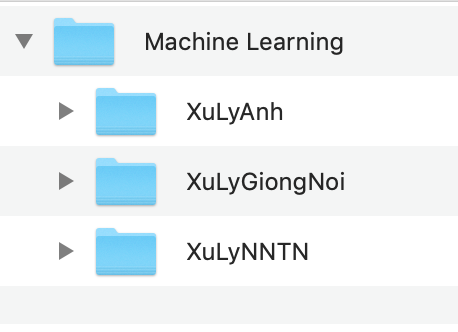
\includegraphics[width=0.5\textwidth]{img/phancapclasses.png}
\end{figure}

trong đó mỗi quan hệ giữa các lớp được mô tả như sau:

\begin{table}[H]
\centering
\begin{tabular}{|l|l|}
\hline
\textbf{SuperClass} & \textbf{SubClass} \\ \hline
Machine Learning    & XuLyAnh           \\ \hline
Machine Learning    & XuLyGiongNoi      \\ \hline
Machine Learning    & XuLyNNTN          \\ \hline
\end{tabular}
\end{table}

\subsection{Tập hợp $R_{KK}$ các quan hệ giữa các keyphrase}
Một quan hệ hai ngôi trên K ($K \neq \emptyset $) là một tập hợp con của $K \times K$ nghĩa là một tập các cặp keyphrase thuộc K và $R_{RR} = \{ r\ |\ r \subseteq K \times K \}$

Trong phạm vi đề tài ta chỉ xét các loại quan hệ sau:

\begin{table}[H]
\centering
\begin{tabular}{|l|l|l|}
\hline
\textbf{} & \textbf{Quan hệ ngữ nghĩa} & \textbf{Mô tả}           \\ \hline
r1        & Đồng nghĩa                 & A đồng nghĩa với B       \\ \hline
r2        & Viết tắt                   & A là dạng viết tắt của B \\ \hline
r3        & Cùng lớp                   & A cùng lớp với B         \\ \hline
\end{tabular}
\end{table}

\begin{itemize}
    \item \textbf{Quan hệ đồng nghĩa r1}: hai keyphrase có quan hệ \textit{đồng nghĩa} nếu chúng cùng nghĩa và thay thế được cho nhau trong một ngữ cảnh nào đó. \\ 
    Ví dụ: keyphrase "công nghệ phần mềm" có quan hệ \textit{đồng nghĩa} với keyphrase "kỹ thuật phần mềm"
    \item \textbf{Quan hệ Viết tắt r2}: hai keyphrase có quan hệ \textit{viết tắt} nếu chúng cùng nghĩa với nhau và thay thế được cho nhau trong một ngữ cảnh nào đó. \\
    Ví dụ: keyphrase "CSS" 
    \item \textbf{Quan hệ Cùng lớp r3}: keyphrase a có quan hệ \textit{cùng lớp} với keyphrase b nếu có một lớp $C_{i}$ sau cho $a \in C_{i}$ và $b \in C_{i}$. \\
    Ví dụ: keyphrase \textit{"Javascript"} có quan hệ cùng lớp với keyphrase \textit{"Typescript"}.
\end{itemize}

\section{Tìm kiếm theo ngữ nghĩa}

\subsection{Công cụ xây dựng Ontology}

Protégé là công cụ phần mềm biên tập ontology mã nguồn mở (được phát triển tại Trường ĐH Stanford) sử dụng đối với việc xây dựng các hệ thống thông minh. Protégé được hỗ trợ bởi cộng đồng lớn bao gồm: các viện nghiên cứu, các tổ chức chính phủ và những người sử dụng cộng tác. Các đơn vị, cá nhân này sử dụng Protégé để xây dựng các giải pháp dựa trên tri thức trong các lĩnh vực chuyên sâu như là: y sinh học, thương mại điện tử và mô hình hóa tổ chức.

Chuẩn ngôn ngữ được sử dụng nhiều nhất để xây dựng ontology hiện nay là OWL\cite{antoniou2004web} được phát triển bởi W3C. Giống như Protégé, OWL có thể mô tả các khái niệm nhưng nó cũng đưa ra các cách thức mới. Nó bao gồm tập rất nhiều các phép toán, ví dụ: phép giao (intersection), phép hợp (union) và phép phủ định (negation). Nó dựa trên một mô hình lo-gic khác giúp nó có thể định nghĩa các khái niệm giống như cách mà các khái niệm đó đã được mô tả.

\subsection{Công cụ lập chỉ mục và tìm kiếm - Apache Solr}

Apache Solr là một nền tảng full-text search mã nguồn mở dựa trên Apache Lucence. Lucene là một thư viện được viết bằng Java dùng để phân tích, đánh chỉ mục (indexing) và tìm kiếm thông tin được phát triển đầu tiên bởi Doug Cutting vào năm 2000. Cutting đồng thời cũng là tác giả của Hadoop lúc ông đang làm việc cho Yahoo vào năm 2005. Solr không hoàn toàn là một RESTful interface của Lucene mà là sử dụng Lucene như là một component trong toàn bộ hệ thống.

Apache Solr có nhiều thành phần chính, nhưng quan trọng nhất là 2 thành phần: Thành phần tạo chỉ mục và thành phần tìm kiếm.


\begin{figure}[H]
    \centering
    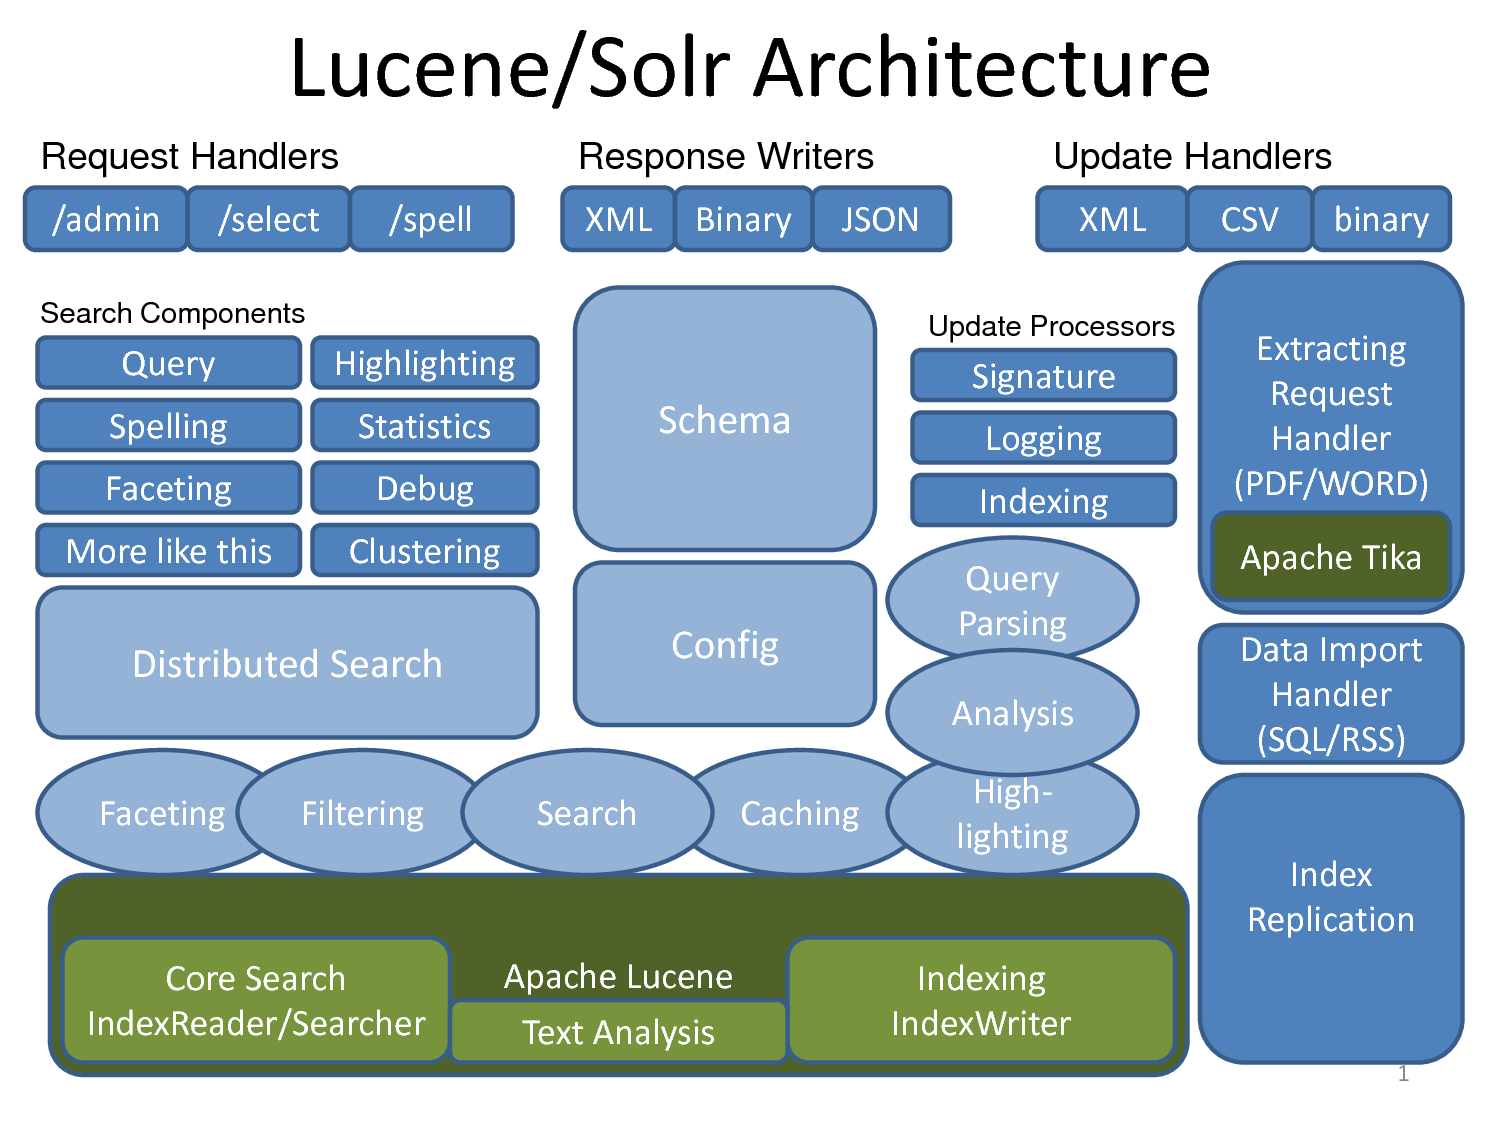
\includegraphics[width=0.8\textwidth]{img/solr-achitecture.png}
    \caption{Các thành phần của Apache Solr}
\end{figure}

\begin{itemize}
    \item \textbf{Thành phần Tạo chỉ mục}: bao gồm các thành phần hỗ trợ xử lý, tạo chỉ mục từ văn bản tài liệu đầu vào và cho ra kết quả là tập chỉ mục phục vụ cho thành phần tìm kiếm. Các component cơ bản bao gồm:
    \begin{itemize}
        \item \textit{Directory}: định nghĩa vùng nhớ, RAM nơi lưu chỉ mục.
        \item \textit{Document và Field}: định nghĩa tài liệu và các trường thông tin của tài liệu cho việc lập chỉ mục, dùng cho việc trả kết quả cho tìm kiếm.
        \item\textit{Analyzer}: thực hiện chức năng xử lý và tách văn bản để lấy nội dung, chuẩn hóa, loại bỏ từ không cần thiết, ... hỗ trợ cho bước lập chỉ mục. \\
        Analyzer đóng vai trò khảo sát các trường văn bản để tạo ra một token stream. Ví dụ: \textit{WhitespaceAnalyzer} xử lý phân tích văn bản thành những token dựa trên khoảng trắng. Câu \textit{"The quick brown fox jump over the lazy dog"} sẽ được phân tích thành các tokens: \textit{[The] [quick] [brown] [fox] [jump] [over] [the] [lazy] [dog]}.
        
        \item\textit{Tokenizer} Nếu như Analyzer tạo ra các token streams/input stream, thì Tokenizer chia nhỏ các stream đó thành những tokens (đơn vị nhỏ nhất để index, có thể là từ hay ký tự). Các ký tự trong input stream có thể bị bỏ qua như các ký tự không nhìn thấy được (whitespace như khoảng trắng, tab) hay các dấu phân cách (delimiter như dấu phẩy, dấu chấm).

        \item\textit{IndexWriter} thực hiện việc tạo mới, mở chỉ mục, thêm hoặc cập nhật nội dung chỉ mục. Đầy là thành phần chính trong thành phần tạo chỉ mục.
    \end{itemize}
    
    \item\textbf{Thành phần Tìm kiếm} bao gồm các thành phần chức năng phục vụ cho việc xử lý tìm kiếm từ yêu cầu người dùng. Solr hỗ trợ nhiều loại truy vấn khác nhau, cho phép tìm theo trường thông tin hay các thiết lập nâng cao như sắp xếp kết quả, giới hạn thời gian hoặc số lượng kết quả, ... \\
    Các chức năng cơ bản gồm:
    \begin{itemize}
        \item\textit{Term}: là đơn vị cơ bản của tìm kiếm, gồm tên và giá trị tương ứng.
        \item\textit{Query} gồm nhiều loại truy vấn, chứa nhiều phương thức, thiết lập chỉ số Boost nhằm giúp xác định truy vấn con nào quan trọng hơn.
        \item\textit{IndexSearcher} tìm kiếm trên tập chỉ mục \textit{IndexWriter} tạo ra.
    \end{itemize}
\end{itemize}

\subsection{Quá trình thiết lập}

\begin{itemize}
    \item Xây dựng tập chỉ mục tìm kiếm
    \begin{itemize}
        \item Mô hình hóa nội dung với Apache Solr
        \item Tiến trình lập chỉ mục
    \end{itemize}
    
    \item Tìm kiếm trên tập chỉ mục
\end{itemize}

\chapter{Cài đặt}

\section{Yêu cầu và chức năng của hệ thống}

Yêu cầu hệ thống tìm kiếm:
\begin{itemize}
    \item Hỗ trợ tìm kiếm theo chức năng thông thường và tìm kiếm theo ngữ nghĩa.
    \item Có một ontology mô tả tri thức lĩnh vực sách CNTT.
    \item Kết quả đáp ứng được nhu cầu tìm kiếm của người dùng.
\end{itemize}

Hệ thống cho phép tìm kiếm theo các cách thức sau:
\begin{enumerate}
    \item Tìm kiếm so trùng dựa vào mọi từ người dùng nhập vào. Kết quả trả về bao gồm tài liệu có các thành phần sau chứa từ khóa tìm kiếm: tiêu đề sách, tên tác giả, tập từ khóa tài liệu.
    \item Tìm kiếm không so trùng chính xác tuyệt đối từ khóa người dùng nhập vào. Hệ thống sẽ tách câu, tách từ, chọn lọc bổ sung các từ khóa sử dụng ontology. Sau đó dùng các từ khóa này để so trùng như cách 1.
\end{enumerate}


\section{Kiến trúc hệ thống}
Kiến trúc hệ thống như sau:

\begin{figure}[H]
    \centering
    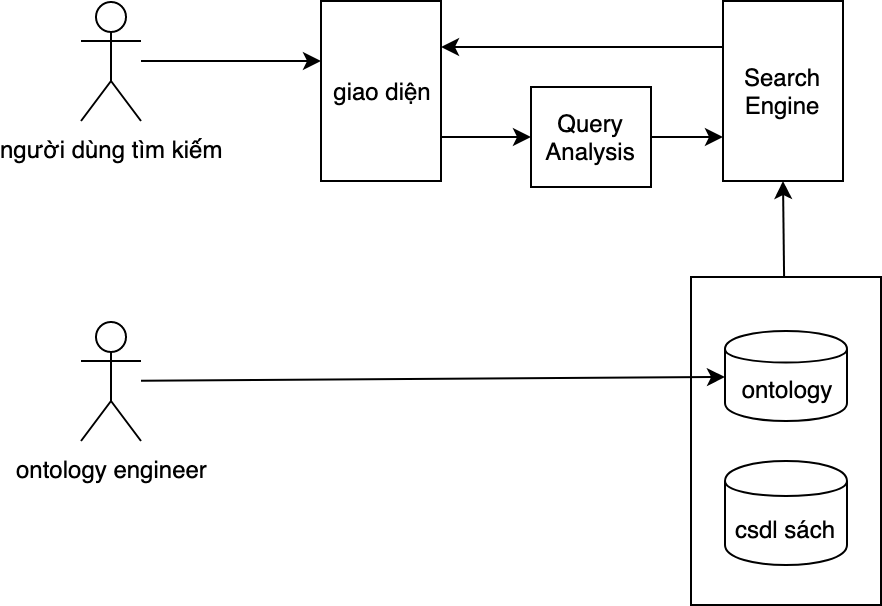
\includegraphics[width=0.8\textwidth]{img/sys_design.png}
    \caption{Kiến trúc hệ thống tìm kiếm ngữ nghĩa với Ontology}
\end{figure}

Mô tả các thành phần trong hệ thống:
\begin{itemize}
    \item \textbf{Database}: cơ sở dữ liệu của toàn hệ thống bao gồm \textit{CSDL SACH} lưu trữ thông tin sách cho hệ thống và \textit{CSDL ONTOLOGY} là ontology cho sách lĩnh vực CNTT.
    \item \textbf{Giao diện}: giao tiếp giữa người dùng và hệ thống.
    \item \textbf{Query Analysis}: tiếp nhận thông tin từ \textbf{Giao diện} chuẩn hóa thông tin sau đó đưa thông tin đến \textbf{Search Engine} của hệ thống.
    \item \textbf{Search Engine}: bộ tìm kiếm sẽ nhận thông tin theo cấu trúc đặc tả từ Query Analysis sau đó thực hiện tìm kiếm, trả kết quả về Giao diện.
    
\end{itemize}

\section{Cài đặt}

Các bước cài đặt bao gồm:
\begin{itemize}
    \item Xây dựng Ontology cho ứng dụng.
    \item Xây dựng thành phần tạo chỉ mục.
    \item Xây dựng thành phần xử lý câu truy vấn và truy vấn dữ liệu dựa trên yêu cầu truy vấn người dùng.
\end{itemize}

\subsection{Xây dựng Ontology}
Các khái niệm được sử dụng trong cơ sở tri thức Ebook là những khái niệm thuộc lĩnh vực giáo dục, được trính ra từ các sách thu thập được trên hệ thống. Báo cáo chỉ tập trung phục vụ tra cứu cho một nhóm nhỏ sách ebook thuộc lĩnh vực CNTT, nên sẽ xây dựng ontology dựa trên dữ liệu sách này.

Ontology trong báo cáo này được rút trích từ mục lục các quyển sách phổ biến trên hệ thống. Các công việc bao gồm thực hiện việc phân loại và rút trích keyphrase từ mục lục, công việc được thực hiện một cách thủ công.

\subsubsection{Thiết kế lớp}
Từ các dữ liệu thu thập được, đề tài đưa ra 7 lớp như sau:
\begin{enumerate}
    \item \textit{TacGia}: lớp tổng quan về tác giả.
    \item \textit{Sach}: lớp tổng quan về sách.
    \item \textit{Keyphrase}: lớp tổng quan về Keyphrase. Gồm các lớp con sau:
    \item \textit{CNTT}: lớp các keyphrase về sách chuyên ngành công nghệ thông tin.
    \item \textit{ML}: lớp các keyphrase về sách chuyên ngành trí tuệ nhân tạo Machine Learning.
    \item \textit{ThietKeWeb}: lớp các keyphrase về sách thiết kế Website.
    \item \textit{CSDL}: lớp các keyphrase về sách cơ sở dữ liệu.
\end{enumerate}

\subsubsection{Thuộc tính lớp}
Các thuộc tính lớp được xây dựng cho ứng dụng dựa trên chuẩn từ vựng Dublin Core và được bổ sung thêm:


\begin{itemize}
    \item\textit{ma\_sach}: mã sách trên hệ thống.
    \item\textit{tieu\_de}: tiêu đề sách ebook.
    \item\textit{ten\_tg}: tiêu tác giả.
    \item\textit{key\_phrase}: danh sách keyphrase biểu diễu nội dung sách.
\end{itemize}


\subsubsection{Các mối quan hệ}
Xây dựng các mối quan hệ bao gồm:

\begin{itemize}
    \item Quan hệ liên quan giữa các lớp:
    \begin{itemize}
        \item Quan hệ giữa Sách và Tác giả: Sach \textbf{coTacGia} TacGia
        \item Quan hệ giữa Tác giả và Sách: TacGia \textbf{laTacGiaCua} Sach
        \item Quan hệ giữa Sách và Tác Giả Phụ: TacGia \textbf{coTacGiaPhu} Sach
        \item Quan hệ giữa Sách và Keyphrase: Sach \textbf{coKeyphrase} Keyphrase
        \item Quan hệ giữa Keyphrase và Sách: Keyphrase \textbf{coKeyphrase} Sach. 
    \end{itemize}
    
    \item Quan hệ giữa các keyphrase:
    \begin{itemize}
        \item Quan hệ đồng nghĩa
        \item Quan hệ viết tắt
        \item Quan hệ cùng lớp  
    \end{itemize}
    
    \item Quan hệ phân cấp trên lớp
    
    \begin{figure}[H]
        \centering
        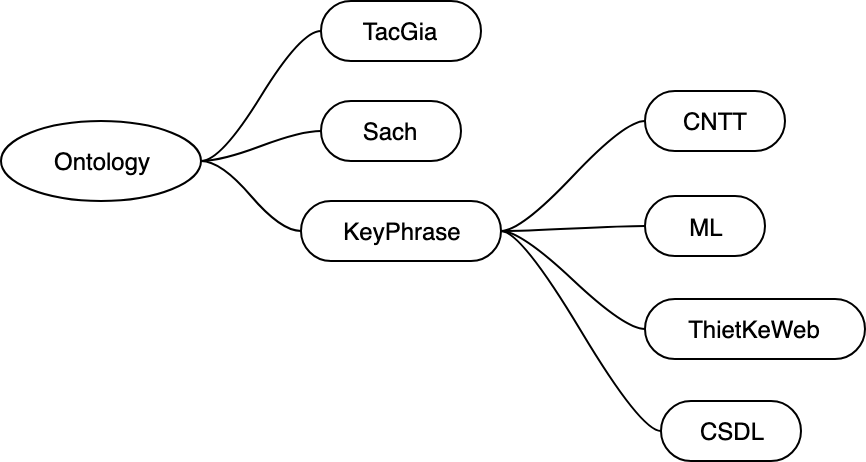
\includegraphics[width=0.8\textwidth]{img/cay_phan_cap.png}
        \caption{Minh họa các quan hệ phân cấp trên lớp}
        \label{fig:quan_he_phan_cap}
    \end{figure}
    
    % Bảng mô tả các lớp:
    
    
\end{itemize}



\subsection{Xây dựng các thành phần tạo chỉ mục}
Thành phần tạo chỉ mục bao gồm các chức năng chính như chỉ định dữ liệu lập chỉ mục, thực hiện phân tích tài liệu, tạo chỉ mục và lưu trữ. Thành phần này kế thừa từ thư viện Apache Solr và Lucene. 

\subsection{Xây dựng thành phần truy vấn}

Thành phần truy vấn gồm các chức năng chính như: nhận thông tin truy vấn, chuyển đổi từ truy vấn và tìm kiếm, hiển thị kết quả trả về. Thành phần biên dịch truy vấn và tìm kiếm cũng kế thừa từ Apache Solr. Quy trình tổng quát như hình \ref{fig:mo_hinh_tim_kiem}.


   \begin{figure}[H]
        \centering
        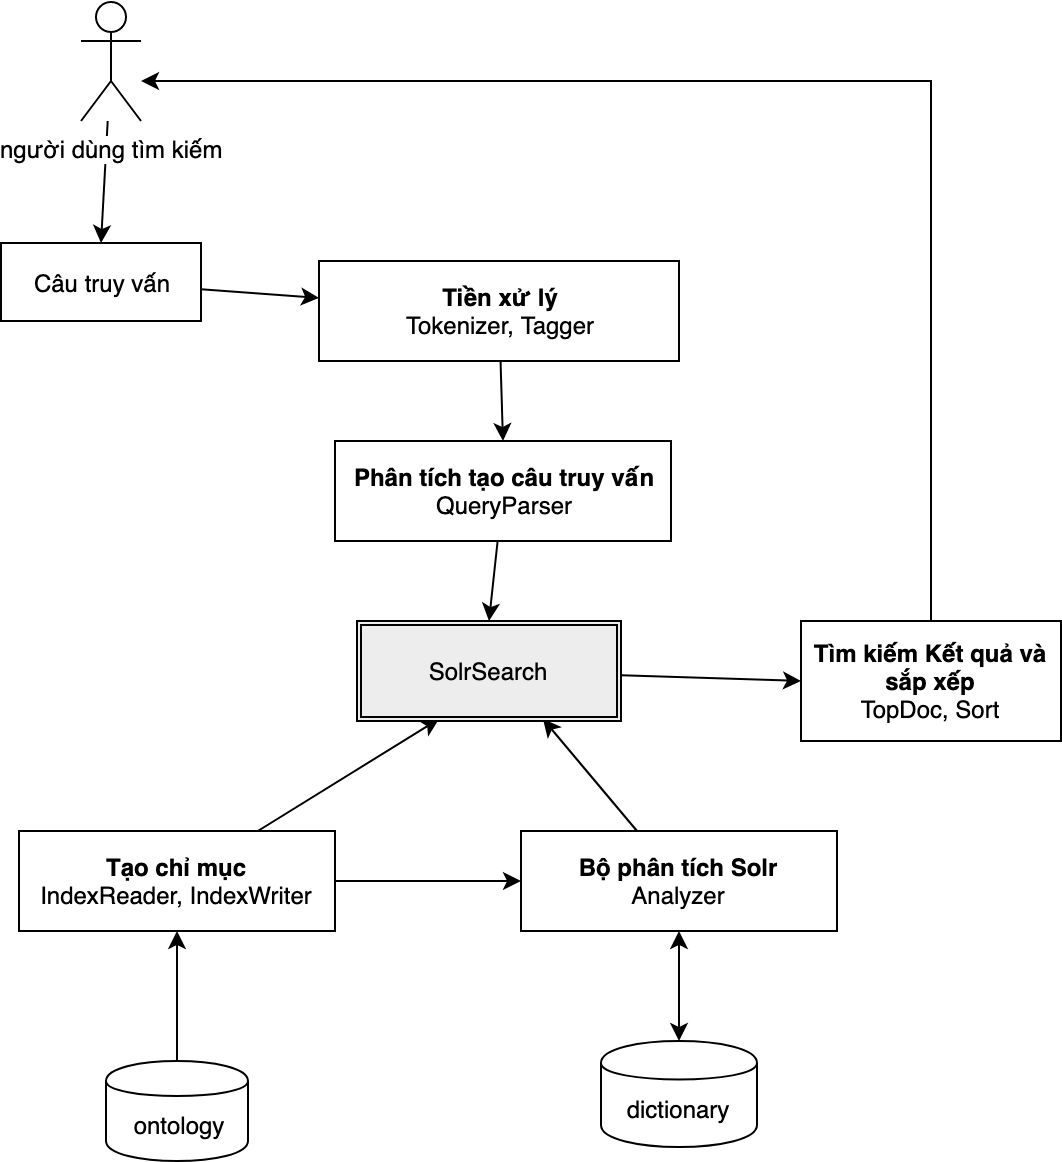
\includegraphics[width=0.8\textwidth]{img/so_do_he_thong.png}
        \caption{Quy trình xử lý trên hệ thống tìm kiếm}
        \label{fig:mo_hinh_tim_kiem}
    \end{figure}
    
    
\begin{itemize}
    \item \textbf{Chuẩn bị dữ liệu cho hệ thống tìm kiếm thực hiện qua các bước}
    \begin{enumerate}
        \item Đọc file ontology
        \item Tạo cây dữ liệu từ ontology: \textit{CreateNodes}
        \item Tạo chi mục tìm kiếm: \textit{IndexReader, IndexWriter}
    \end{enumerate}
    
    \item \textbf{Quy trình xử lý tìm kiếm hiện qua các bước}
    \begin{enumerate}
        \item Người dùng nhập câu
        \item Tiền xử lý: tách từ, gán nhãn cho câu truy vấn
        \item Xây dựng cây truy vấn theo chuẩn Apache Solr: \textit{QueryParser}
        \item Thực hiện tìm kiếm: \textit{SolrSearch}
        \item Đánh giá kết quả và sắp xếp theo độ đo: \textit{TopDoc, TopDoc.Sort}
        \item Hiển thị kết quả cho người dùng.
    \end{enumerate}
    
    
    \item \textbf{Thuật toán}
    \begin{itemize}
        \item Thuật toán xây dựng cấu trúc tìm kiếm từ file Ontology
        
        \begin{lstlisting}[language=Python,numbers=left,frame=single, basicstyle=\ttfamily\small]
loadOntology(iw IndexWriter, o Sach):
    iw.MaSach = getMaSach(s)
    iw.TuaSach = getTuaSach(s)
    
    while KeyPhrase in getKeyPhrase(s):
        iw.KeyPhase[] = KeyPhrase
        
    while TacGia in getTacGia(s):
        iw.TacGia[] = TacGia
        \end{lstlisting}

    \item Lấy toàn bộ thông tin sách và load vào Solr Index

 \begin{lstlisting}[language=Python,numbers=left,frame=single, basicstyle=\ttfamily\small]
buildIndex():
    // Khoi tao IndexWriter
    IndexWrite iw = IndexWrite{}
    
    // Lay danh sach ebooks tu Database
    Sach[] books = getBooksFromDB()
    
    // Load vao index Solr
    while book in books:
        loadOntology(iw, book)
        \end{lstlisting}

    \end{itemize}
    
    
    \item \textbf{Giao diện tìm kiếm Apache Solr}
    
    Hình \ref{fig:solr_client} thể hiện giao diện tìm kiếm của Apache Solr Client dưới dạng web, kết quả trả về có thể ở dạng JSON hoặc XML, dễ dàng tích hợp vào các hệ thống Web hoặc Application khác.
     
     \begin{figure}[H]
        \centering
        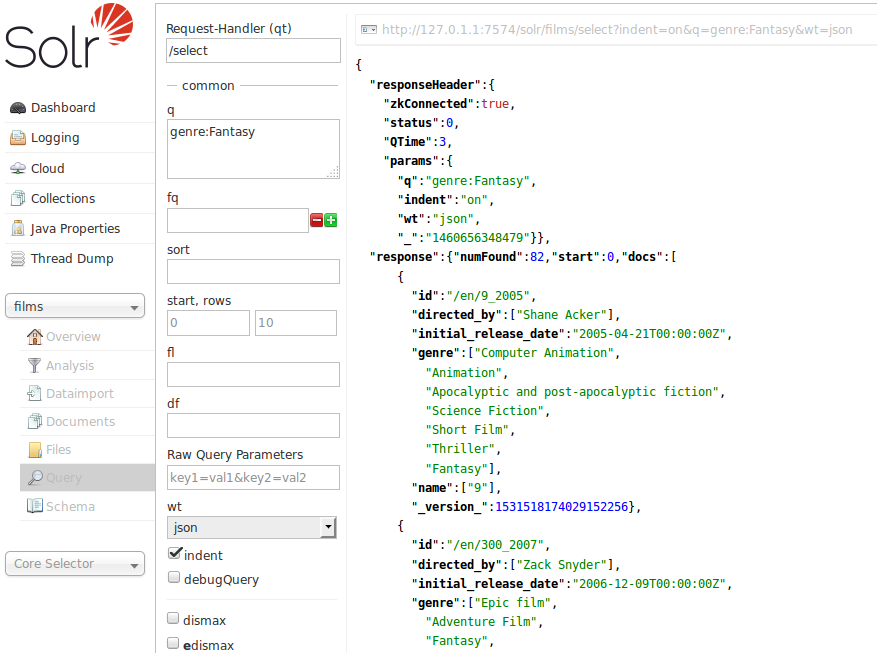
\includegraphics[width=1\textwidth]{img/solr.png}
        \caption{Giao diện tìm kiếm Apache Solr Client}
        \label{fig:solr_client}
    \end{figure}
    
    
\end{itemize}

\chapter{Kết luận}

\section{Kết quả đạt được}

Qua kết quả ta thấy tầm quan trọng của việc biểu diễn tri thức và ứng dụng của nó trong thực tiễn, cụ thể trong báo cáo này giúp tăng độ chính xác cho hệ thống tìm kiếm bằng cách bổ sung ngữ nghĩa. Báo cáo có những kết quả như sau:

\begin{itemize}
    \item Hiểu cách xây dựng một ontology từ dữ liệu sách ebook.
    \item Ứng dụng ontology vào thư viện chỉ mục và tìm kiếm Apache Solr.
    \item Tìm kiếm tài liệu bằng cách chọn lọc lại từ khóa trong câu truy vấn của người dùng.
\end{itemize}

\section{Hạn chế}

Thời gian có hạn nên báo cáo còn khá nhiều chức năng chưa thực hiện:
\begin{itemize}
    \item Chưa cho phép truy cập, hiệu chỉnh Ontology
    \item Chưa tập hợp được kiến thức chuyên gia để xây dựng hệ Ontology.
    \item Chỉ tập trung xây dựng ứng dụng một lĩnh vực cụ thể.
    \item Chỉ kiểm tra trên những câu truy vấn cơ bản, phụ thuộc vào các tập keyphrase đã được xây dựng sẵn trong ontology.
\end{itemize}

\section{Định hướng phát triển}

Để phát triển và đưa vào thực tiễn, cần:
\begin{itemize}
    \item Xây dựng hoàn thiện Ontology từ chuyên gia.
    \item Mở rộng sang các miền, chuyên ngành sách khác.
\end{itemize}
% \include{chuong_6}
 
\bibliographystyle{unsrt} % bibliography style
\renewcommand{\bibname}{Tài liệu tham khảo} % changes default name Bibliography to References
\bibliography{ref} % References file

\end{document}
